\chapter{Konstrukcja urządzenia}
\label{cha:constr}
W~tym rozdziale, po wybraniu rodzaju konstrukcji oraz platformy sprzętowej, autor przedstawia zastosowane komponenty oraz generalną konstrukcję mechaniczną  i~elektryczną budowanego projektu.
\section{Zastosowane komponenty}
\label{sec:komponenty}
Aby skonstruować kompletny system pasywno-aktywnego tłumienia hałasu, autor zbudował swój projekt na bazie prostych, komercyjnych nauszników tłumiących ze sklepu z~artykułami BHP, stosowanych w~budownictwie lub przemyśle (rys. \ref{fig:nauszniki_bhp}).
\begin{figure}[h!]
	\centering
	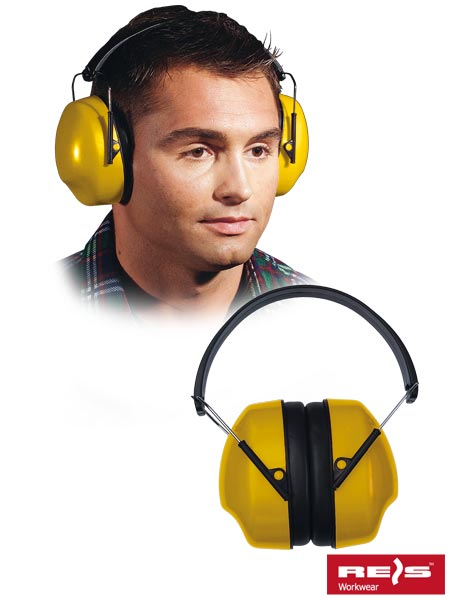
\includegraphics[scale=0.4]{../Assets/nauszniki_bhp.png}
	\caption{Użyte w~projekcie nauszniki ochronne.\\ Źródło: Copyright \textsuperscript{\textcopyright} by REIS GROUP}
	\label{fig:nauszniki_bhp}
\end{figure}

Nauszniki te stanowią część tłumiącą pasywnie. Do stworzenia i~zaimplementowania części aktywnej układu zastosowano wymienione poniżej elektroniczne elementy analogowe oraz cyfrowe, przy czym elementy cyfrowe są wymienione każdy z~osobna, pomimo iż stanowią integralne podzespoły mikrokontrolera.
\begin{enumerate}
	\item Analogowe:
	\begin{itemize}
		\item Pojemnościowy mikrofon elektretowy typu CMA-4544PF-W (rys. \ref{fig:mikrofony_max4466}) -- dwie sztuki\\
		W~urządzeniu zamontowano jeden główny (feedforward) na zewnątrz muszli oraz jeden odsłuchowy (feedback) wewnątrz muszli słuchawki.
		\item Przedwzmacniacz mikrofonowy typu Adafruit MAX4466 -- dwie sztuki\\
		\begin{figure}[h!]
			\centering
			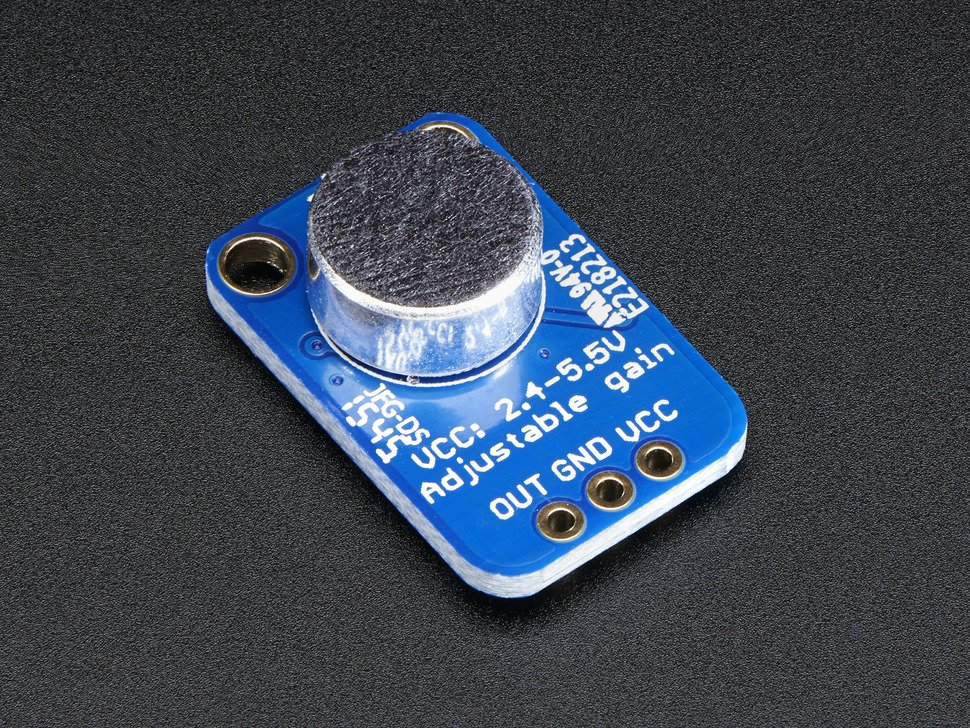
\includegraphics[scale=0.2]{../Assets/adafruit_max4466.png}
			\caption{Użyte w~projekcie mikrofony z~przedwzmacniaczami.\\ Źródło: https://cdn-shop.adafruit.com/970x728/1063-03.jpg}
			\label{fig:mikrofony_max4466}
		\end{figure}
		Wzmacniacz operacyjny zoptymalizowany przez producenta pod kątem wykorzystania z~mikrofonami. Autor zakupił przedwzmacniacz połączony przez producenta z~wyżej wymienionym mikrofonem w~ramach jednej płytki (rys. \ref{fig:mikrofony_max4466}). Należy pamiętać o~przesunięciu fazy sygnału -- jednak ten problem powinien zostać rozwiązany przez filtr adaptacyjny.
		\item Wzmacniacz audio klasy D typu Adafruit PAM8302 (rys. \ref{fig:pam8302})\\
		\begin{figure}[h!]
			\centering
			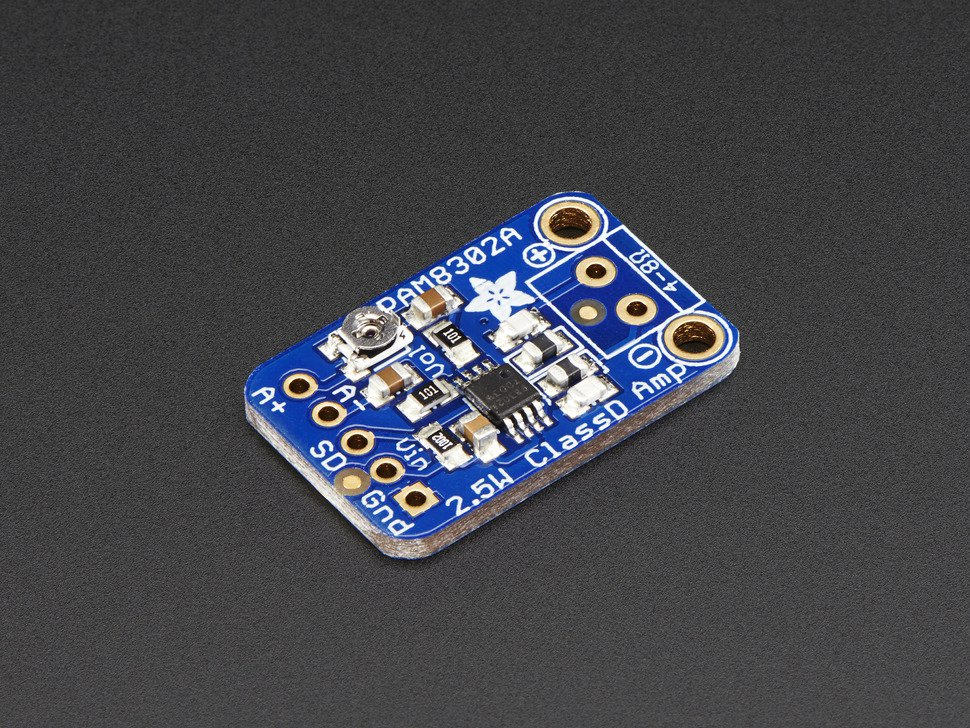
\includegraphics[scale=0.2]{../Assets/wzmacniacz_pam8302.png}
			\caption{Użyty w~projekcie wzmacniacz audio.\\ Źródło: https://cdn-shop.adafruit.com/970x728/2130-01.jpg}
			\label{fig:pam8302}
		\end{figure}
		Ten wzmacniacz monofoniczny o~mocy \SI{2.5}{\W} przeznaczony jest do współpracy z~głośnikami o~impedancji od \SI{4}{} do \SI{8}{\ohm}. Producent deklaruje sprawność w~zakresie 85-88\% \cite{speakeropamp} oraz współczynnik zawartości harmonicznych i~szumów (THD+N) wynoszący 10\%.
		\item Głośnik typu MG15 o~mocy \SI{0.1}{\W} oraz impedancji \SI{8}{\ohm} (rys. \ref{fig:mg15})\\
		\begin{figure}[h!]
			\centering
			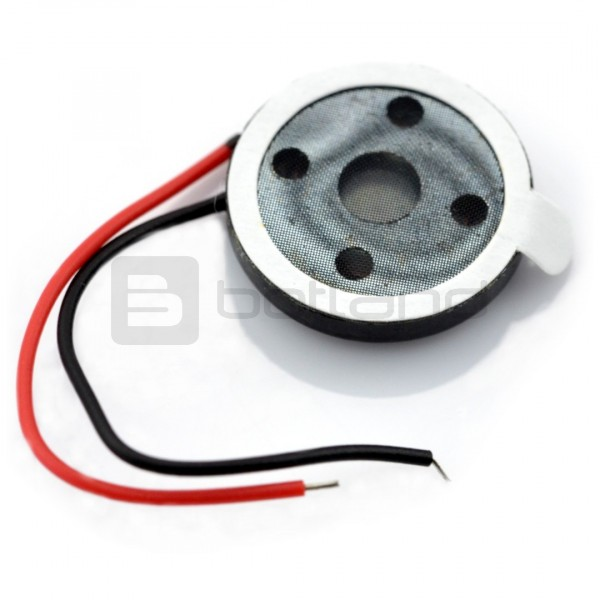
\includegraphics[scale=0.1]{../Assets/glosnik_mg15.png}
			\caption{Użyty w~projekcie głośnik.\\ Źródło: https://botland.com.pl/49567-thickbox\_default/glosnik-mg15-01w-8ohm-15x4mm.jpg}
			\label{fig:mg15}
		\end{figure}
		\item Filtr dolnoprzepustowy (antyaliasingowy) -- dwie sztuki\\
		Zanim sygnał zostanie dostarczony do przetwornika A/C, należy zapewnić, by jego częstotliwość nie przekroczyła częstotliwości Nyquista\footnote{Jest to połowa częstotliwości próbkowania sygnału. Przekroczenie jej przez nieodfiltrowany sygnał powoduje pokrycie się dwóch, różnych od siebie sygnałów. Przykład aliasingu: Dla częstotliwości Nyquista równej \SI{1000}{\Hz}, nieodfiltrowany sygnał \SI{3100}{\Hz} zostałby odczytany jako sygnał \SI{100}{\Hz}.}. Pozwala to uniknąć błędnego zakodowania sygnału w~dziedzinie cyfrowej. W~pracy zastosowano pasywny filtr dolnoprzepustowy RC pierwszego rzędu.
		%\item Filtr dolnoprzepustowy 2 (rekonstrukcyjny, anti-imagingowy)\\
		%Podobnie jak na wejściu do części cyfrowej układu, również na jej wyjściu należy umieścić filtr dolnoprzepustowy (na wyjściu przetwornika C/A) -- aby zapobiec wtłaczaniu wyższych harmonicznych do głośnika.
	\end{itemize}
	\item Cyfrowe:
	\begin{itemize}
		\item Przetwornik analogowo-cyfrowy -- dwie sztuki\\
		Autor zdecydował się użyć dwóch osobnych przetworników (wchodzących w~skład mikrokontrolera) do akwizycji sygnału z~mikrofonów, aby uniknąć przesłuchów, które mogłyby się pojawić w~przypadku użycia pojedynczego przetwornika. Przyczyną przesłuchów jest zwykle multiplekser analogowy wybierający kanały wejściowe przetwornika A/C. Takie rozwiązanie zmniejsza też nieznacznie opóźnienia w~przetworzeniu sygnału, gdyż można wtedy skonfigurować przetworniki w~trybie mierzenia pojedynczego kanału, a~nie skanowania dwóch po kolei. Przetwornik realizuje algorytm SAR\footnote{Sukcesywna Aproksymacja (ang. Successive Approximation Register, inaczej próbkowanie bitowe)}.\\
		Warto zauważyć, że przetworniki dostępne na płytce użytej przez autora mają rozdzielczość 12~bitów, co pozostawia pewne pole do poprawy projektu i~wyboru komponentów, ale jednocześnie zapewnia wystarczający poziom dokładności dla potrzeb prototypowania układu.
		\item Timer (Licznik)\\
		Do zadania wyznaczenia stałego kroku próbkowania wybrano timer~3. Jest to podstawowy licznik mikrokontrolera, bez dodatkowych funkcjonalności (jakie posiada chociażby timer~1). Odmierzenie zadanego interwału czasowego sygnalizowane jest wewnętrznie jako zdarzenie, które wychwytuje przetwornik A/C. Jego konfiguracja została opisana w~sekcji~\ref{sec:configuration}.
		\item Kontroler DMA (Direct Memory Access) -- dwie sztuki\\
		Jeden z~kontrolerów użyty jest do transferu danych z~przetworników~A/C do pamięci mikrokontrolera STM32, zaś drugi - do transferu (po przeprowadzeniu eksperymentu) wartości nastaw filtra LMS z~pamięci do kontrolera UART. Transfer w~pierwszym przypadku dokonywany jest w~trybie ciągłym, a~więc po każdym przerwaniu do DMA, zgłoszonym przez przetwornik na końcu konwersji. W~drugim przypadku, transfer wywoływany jest po wciśnięciu przez testera przycisku na płytce prototypowej lub wysłaniu odpowiedniej komendy z~komputera~PC.
		\item NVIC (Nested Vectored Interrupt Controller)\\
		Kontroler przerwań (zagnieżdżonych), który przyspiesza ich obsługę.
		\item USART (Universal Synchronous/Asynchronous Receiver/Transmitter)\\
		Komponent odpowiedzialny za transmisję danych w~trybie full-duplex pomiędzy mikrokontrolerem a~dowolnym innym urządzeniem obsługującym protokół komunikacji USART. Połączenie UART z~komputerem nie wymagało użycia konwertera USB-UART, gdyż programator/debugger ST-Link, obecny na użytej płytce NUCLEO, posiada podłączone wyprowadzenia UART z~mikrokontrolera. Dane odebrane przez programator są bezpośrednio przekazywane do kontrolera USB, który już jest podłączony do komputera PC. Zatem przy użyciu jednego połączenia można zarówno zasilać urządzenie, programować je, debuggować, jak i~również odbierać z~niego dane.
		\item Rdzeń mikrokontrolera\\
		Główna jednostka obliczeniowa.
		\item FPU (Floating Point Unit)\\
		Jednostka dedykowana do obliczeń zmiennoprzecinkowych na liczbach 32-bitowych (a~więc typu float). Znacznie podnosi precyzję obliczeń na ułamkach i~przyspiesza działanie całego układu jeżeli takich działań jest dużo. Należy jednak pamiętać, że operuje jedynie na danych pojedynczej precyzji. 
		\item Przetwornik cyfrowo-analogowy\\
		Do celu prototypowego użyto jednego kanału wyjściowego, aby przetestować działanie systemu w~jednolitej, odgrodzonej przestrzeni sferycznej. Konwersja sygnału na postać analogową następuje automatycznie, bez oddzielnego inicjowania, przy każdej wykrytej zmianie słowa bitowego wpisanego przez program do rejestru danych wyjściowych przetwornika DAC. Dane są wpisywane do tego rejestru po każdym skończonym cyklu obliczeniowym.
	\end{itemize}
\end{enumerate}

\section{Schemat i konfiguracja układu}
\label{sec:config}
Uproszczony schemat w~wersji graficznej został przedstawiony przez autora na rysunku \ref{fig:schemat1}. Podstawową zasadą działania systemu jest:
\begin{enumerate}
	\item Akwizycja sygnału przez dwa mikrofony: główny oraz odsłuchowy.
	\item Wzmocnienie sygnału przez przedwzmacniacz mikrofonowy.
	\item Konwersja analogowego sygnału do postaci cyfrowej w~przetworniku ADC.
	\item Transfer danych przez kontroler DMA do pamięci urządzenia.
	\item Odczyt danych (pochodzących z~mikrofonu głównego) z~pamięci i~przetworzenie ich w~filtrze FIR.\\
	Odczyt danych (pochodzących z~mikrofonu odsłuchowego) z~pamięci i~przetworzenie ich w~module strojenia LMS.
	\item Jednoczesne przekazanie danych z~mikrofonu głównego do modułu strojenia filtra LMS.
	\item Przestrojenie filtra na podstawie algorytmu LMS.
	\item Obliczenie odpowiedzi filtra FIR i~przesłanie jej do przetwornika DAC.
	\item Wzmocnienie sygnału przez wzmacniacz audio.
	\item Odtworzenie sygnału wytłumiającego przez głośnik.
\end{enumerate}
\begin{figure}[h!]
	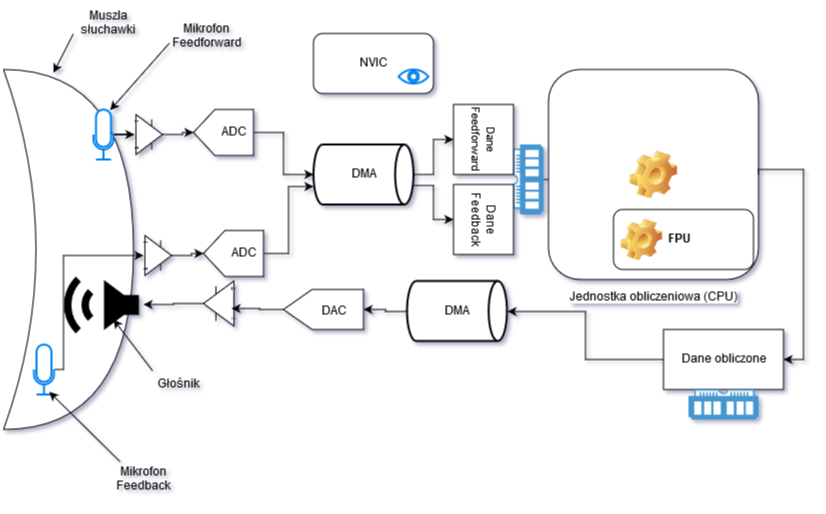
\includegraphics[width=\linewidth]{../Assets/schemat_ukladu.png}	
	\caption{Schemat układu.}
	\label{fig:schemat1}
\end{figure}
Autor pominął pomniejsze elementy, które nie wnoszą szczególnych informacji do opisu pracy. W~kwestii umiejscowienia mikrofonu odsłuchowego autor posłużył się wnioskami przedstawionymi w~artykule dotyczącym aktywnej redukcji hałasu w~zastosowaniach słuchawek tłumiących \cite{ANC4HP}. Autorzy pracy na podstawie widma częstotliwościowego wyznaczyli optymalne położenie mikrofonu i~wykazali, że takim miejscem jest bliskie otoczenie przewodu słuchowego zewnętrznego. Konkretne położenie mikrofonu odsłuchowego ilustruje lokacja nr~8 na rysunku \ref{fig:error_mic_placement} zapożyczonym z~wyżej wymienionej pracy.
Mikrofon odsłuchowy umiejscowiony w~optymalnej pozycji charakteryzuje się zlinearyzowaną odpowiedzią częstotliwościową, co ogranicza błędy pomiarowe, poprawiając precyzję zastosowanego rozwiązania.
\begin{figure}[h!]
	\centering
	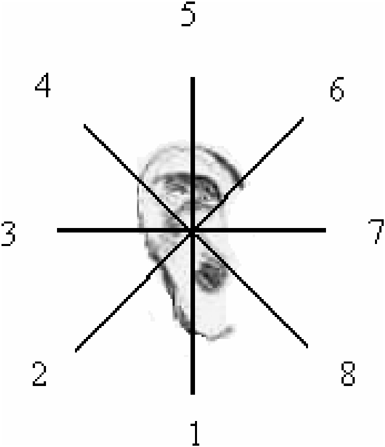
\includegraphics[scale=0.6]{../Assets/error_mic_placement.png}
	\caption{Położenie mikrofonu odsłuchowego odzwierciedla lokacja nr 8.\\ Źródło: \fullcite{ANC4HP}; strona 333}
	\label{fig:error_mic_placement}
\end{figure}

Aby stworzyć odgrodzoną przestrzeń sferyczną, autor postanowił złączyć (ścisnąć) dwie słuchawki użytych nauszników. Pomiędzy słuchawkami umieszczono element dystansowy (długopis), aby zamodelować nieidealne przyleganie słuchawek do głowy potencjalnego użytkownika. Do celów testowych nie będzie potrzebny dodatkowy mikrofon umieszczony w~środku przestrzeni -- zostanie użyty zamontowany już mikrofon odsłuchowy. Dane z~niego zostaną odczytane przy użyciu sondy oscyloskopu.

Aby zasilić prototyp, autor podłączył mikrokontroler poprzez USB do komputera osobistego. Zapewniło to standardowe zasilanie mikrokontrolera na poziomie \SI{3.3}{\V}. Ponadto, celem odseparowania części analogowej od cyfrowej, autor zdecydował się zapewnić osobne zasilanie dla układów analogowych, a~więc mikrofonu wraz z~jego przedwzmacniaczem oraz dla wzmacniacza głośnikowego. Tym samym zredukowane są zakłócenia, które normalnie mogłyby się przenieść z~linii zasilania układu cyfrowego do bardzo wrażliwej na te zakłócenia części analogowej. Zasilanie to, dla mikrofonów, zostało osiągnięte poprzez dołączenie pastylkowych baterii \SI{3}{\V} typu CR2032 do elementów analogowych. Zasilanie przedwzmacniacza z~głośnikiem wymaga użycia nieco innej metody ze względu na dużą moc komponentu -- zwykła bateria nie wystarczyłaby do odpowiednio długotrwałego działania układu. Biorąc pod uwagę prototypowy charakter całego urządzenia oraz konieczność połączenia mikrokontrolera z~komputerem, autor zdecydował się zasilić przedwzmacniacz przy użyciu modułu zasilającego z~płytki stykowej, podłączonego przez zasilacz impulsowy DC \SI{9}{\V} do gniazdka sieciowego. Przyłącze zasilacza nie posiada złącza uziemienia, dlatego po połączeniu wszystkich komponentów w~całym układzie występuje jeden wspólny punkt uziemiający -- jest nim GNDA, czyli masa analogowa mikrokontrolera. Pozwala to uniknąć pętli masy, które miałyby wpływ na jakość sygnału w~urządzeniu. Warto zwrócić uwagę na fakt, że gdyby zasilający wzmacniacz mocy został podłączony przez magistralę USB, to powstałaby pętla masy pomiędzy układem mierzonym a~komputerem pomiarowym, który zasila już zestaw uruchomieniowy z~mikrokontrolerem.